\chapter{Architecture Exploration}\label{models}
This chapter presents the proposed neural network architectures. It starts with a baseline TNN network implemented in \texttt{PyTorch}, which then undergoes a series of hardware-aware adaptions specific to jet tagging. During this process two separate architectures are developed, which differ by the input type and design goal. The first one, referred to as the \textit{ultra-low latency} one, targets the HLF jet representation and aims to achieve the lowest possible latency at the cost of accuracy and AUC values. The second one, called \textit{accuracy-focused}, is based on the constituent list jet representation and trade-offs latency for quality of classification while still remaining within L1T timing constraints.


\section{Base Architecture}
The starting point of this analysis is derived from transformer architecture used in the original paper \cite{44-vaswani2017attention} and recent proof-of-concept used for jet tagging \cite{3-yuan2021constituentnet:}. The overview of the network components can be seen in figure \ref{fig:constituent-net}.

\begin{figure}[hpt!]
  \centering
  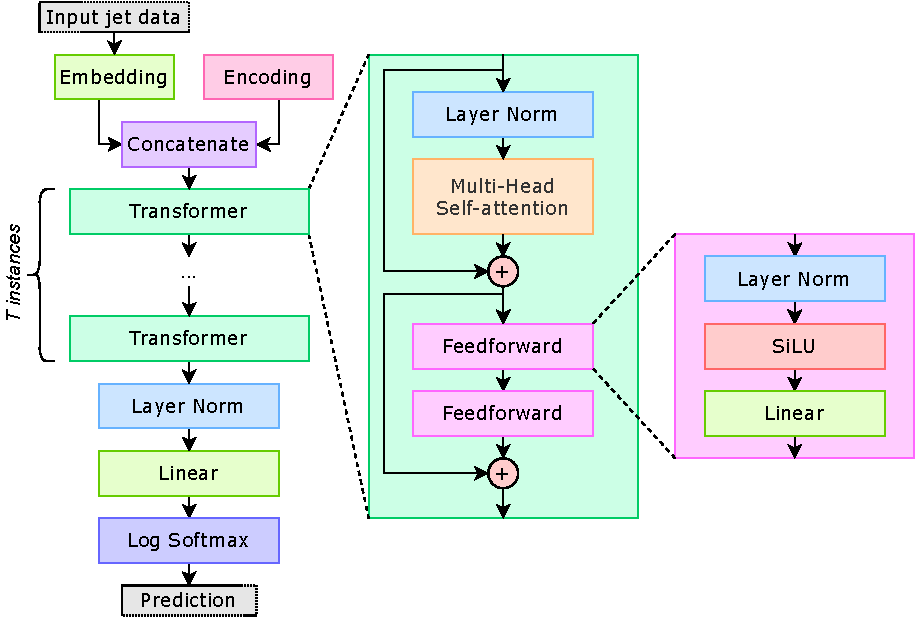
\includegraphics[trim={0cm 0cm 0cm 0cm}, width=0.6\textwidth, center]{models/constituent_net.pdf}
  \caption{Diagram with an overview of the baseline architecture.}
  \label{fig:constituent-net}
\end{figure}

The straight-forward path between model's input and output highlights the sequential nature of transformer which stands in opposition to recurrency present in GRU and LSTM models. While this allows for the aforementioned parallelizability and pipelining on FPGAs, it also poses a challenge of increased hardware footprint and synthesis complexity when compared to recurrent models, where the key components can get reused to meet the resource constraints. To better understand the transformer's complexity, the next subsections derive the equations linking the internal components and explain the involved terminology.


\subsection{Input embedding and Residual Connections}
Although the model lacks any recurrency, the transformer includes two residual connections which have been widely adopted since their successful application in ResNet neural networks \cite{75-kaiming2016deep}. They offer improvements to training time and resulting accuracy \cite{74-szegedy2016inception-v4}, however, they require standardized data dimensionality to ensure the summation can be logically executed. In this project, this is obtained thanks to input embedding, which transforms the input \(\bm{\hat{x^i}} \in \mathbb{R}^{L \times 16} \) into a shape \(\mathbb{R}^{L \times d}\) that is used through the design, as seen in equation \ref{eq:embedding}. The \(d\) size is referred to as the self-attention latent or embedded dimension.

\begin{equation}\label{eq:embedding}
  \bm{\hat{x^i}_{\text{emb}}} = \text{embedding} ( \bm{\hat{x^i}} ) = w_{\text{embed}}\; \bm{\hat{x^i}} + b_{\text{embed}} \in \mathbb{R}^{L \times d}
\end{equation}

This dimensionality change can be conveniently performed using a linear layer, and it has to be remembered that each such layer increased the model learning capacity thanks to the learnable weights and bias. The network's inner dimension \(d\) is treated as a hyperparameter as it influences the model's accuracy and performance, but it has to be noted that the other dimension prevalent in the network comes from the input's number of jet constituents \(L\) (which is set to 1 in case of the HLS representation), meaning that the model is also susceptible to a parameter which cannot be easily tuned.


\subsection{Input Encoding}
Along the embedding, an input encoding is concatenated and fed to the transformer layer. In natural language processing, the encoding is meant to allow the model to benefit from the sequential information of the words in a sentence. It can be obtained from a sinusoidal function using the position index or simply treated as another learnable parameter. The sequential relations are not present in the jet data, because all the jets originate from the same proton-proton collision, hence, the latter approach is used in this project. It is worth mentioning, that from empirical analysis, the learnable encodings have a significant impact on the final results as they represent a trained, hidden state concatenated to all inputs during evaluation, as shown in equation \ref{eq:encoding}. Its impact is especially prevalent for the HLF data (where \(L = 1\)), where the hidden state matched input's dimension and effectively doubles it after concatenation.

\begin{equation}\label{eq:encoding}
  \text{encoding} ( \bm{\hat{x^i}_{\text{emb}}} ) = w_{\text{encoding}} \in \mathbb{R}^{1 \times d} \implies \text{concat} (\bm{\hat{x^i}_{\text{emb}}},\; w_{\text{encoding}}) \in \mathbb{R}^{(L+1) \times d}
\end{equation}

Choosing a learned hidden state is also more efficient for inference in hardware, as the increased training cost associated with back-propagation of this parameter yields a constant set of values that are known during compile-time of the FPGA and can be implemented using a LUT.


\subsection{Normalization and Parameter Extraction}
As layer normalization does not track and gather running mean and variance statistics, this mechanism is implemented on top of the existing \texttt{PyTorch} implementation to facilitate extracting the aggregated statistics after training. These, along with all the learned weights and biases, are extracted and transformed into specific C++ formats supported in HLS using a custom tool developed for this purpose. This allows for directly initializing the FPGA's BRAMs and LUTs with the model parameters, which avoids the need for an interaction with a host machine.

Obtaining the statistics taken for the data before normalization layers can also be viewed as a hardware-aware optimization. This can be explained with the mathematical derivation presented in equation \ref{eq:normalization-optimization}

\begin{equation}\label{eq:normalization-optimization}
  y = \frac{x - E[x]}{\sqrt{Var[x] + \epsilon}} \cdot \gamma + \beta = x \cdot (\frac{\gamma}{\sqrt{Var + \epsilon}}) + (\beta - \frac{\gamma * E}{\sqrt{Var + \epsilon}}) = w \cdot x + b
\end{equation}

By treating the mean \(E[x]\) and variance \(Var[x]\) of input \(x\) as learned parameters, the square root and division operations can be fully omitted by fusing them into the existing \(\gamma\) and \(\beta\) parameters which simplifies the hardware required for the normalization layers. This is especially useful as FPGAs lack dedicated hardware for these computationally expensive operations, which could lead to suboptimal designs being synthesized. Independently of the implementation in this work, a similar idea has been proposed and successfully used as an optimization in the past \cite{46-fan2018real-time}.

The algorithm behind the parameter extraction is rather simple, and the difficulty comes from the domain specific knowledge of handling \texttt{PyTorch} model parameters and generating the correct files for HLS. The break-down of the necessary steps can be seen in algorithm \ref{alg:parameter-extraction}.

\begin{algorithm}
  \caption{Mechanism behind model parameter extraction}\label{alg:parameter-extraction}
  \begin{algorithmic}[1]
    \State $state \gets $load\_state(model)
    \State sort($state$)
    \State $curr\_weight \gets $null
    \For{$param$ in $state$}
      \State $mean \gets $find\_mean(model, param)
      \State $var \gets $find\_var(model, param)

      \If{$param$ is weight}
        \State $curr\_weight \gets $param
        \State $new\_param \gets $update\_weight(param, var)

      \Else
        
        \State $new\_param \gets $update\_bias(param, curr\_weight, mean, var)
      \EndIf
      \State \texttt{save(new\_param)}
    \EndFor
  \end{algorithmic}
\end{algorithm}



\section{Ultra-Low Latency Architecture}
The first of the proposed architectures targets the HLF representation dataset, where each sample is of \(\mathbb{R}^{1 \times 16}\) dimensions, making it a better candidate for an \(N\) times faster inference than the constituent list representation with inputs with \(\mathbb{R}^{N \times 16}\) dimensions. The simpler data means that the network can achieve satisfactory classification results with a lower learning capacity, hence allowing for various simplifications of the base architecture.

\subsection{Simplification and Tuning}
The hypothesis leading the optimization process is that the HLF dataset can be learned by a relatively lower complexity network. The strategy is to start with the accuracy and AUC value of the base architecture and keep applying changes to the network as long as they do lead to significant drops in classification results, with detailed evaluation discussed in 
\cref{evaluation}. Doing so is inherently beneficial for the later FPGA mapping, as even without hardware-aware changes, a simpler model is likely to require less resources and achieve lower latency.

The architecture features that have the highest influence on the overall performance are the size of the latent dimension and number of transformer layer. In the case of the original transformer model \cite{44-vaswani2017attention}, 12 transformer layers are used, split equally into a decoder and encoder parts of the networks. This, along with latent dimension size of 512 shows that jet tagging requires significantly less complexity compared to natural language processing, as the recent ConstituentNet \cite{3-yuan2021constituentnet:} is based on only 3 transformer layers and embedded dimension of 64. However, as the latter network targets a more complex dataset, the first optimization performed in this project yielded a reduction to only a single transformer layer with latent size of 16. The network complexity is directly proportional to the number of layers, while the self-attention complexities shown in \cref{self-attention} can be simplified given the dimensions of \textit{queries}, \textit{keys}, and \textit{values} are shared and equal to \(\in \mathbb{R}^{N \times d}\) in this work, 
as shown in equation \ref{eq:qkv-complexity-time-simple} and \ref{eq:qkv-complexity-space-simple} for time and space respectively.

\begin{equation}\label{eq:qkv-complexity-time-simple}
  \mathcal{O}(h \cdot (N_Q N_K (d_Q + d_V) + d_Q^2 (N_Q + N_K) + d_V^2 N_K + N_Q d_V d_{out}) )) \equiv
  \mathcal{O}(h N d (N + d + d_{out}) ))
\end{equation}

\begin{equation}\label{eq:qkv-complexity-space-simple}
  \mathcal{O}(h \cdot (N_Q (N_K + d_V) + d_Q (N_Q + N_K) + d_V N_K + N_Q d_{out}) )) \equiv
  \mathcal{O}(h N (N + d + d_{out}) ))
\end{equation}

Another successful optimization was simplifying the SiLU to ReLU activations, as in hardware, the latter rely on a single comparator to determine whether to pass input to output directly or set the signal to zero. In contrary, SiLU requires computing the sigmoid function as well as performing a multiplication, which has a non-trivial cost on an FPGA.

Interestingly, the layer normalization was first changed to batch normalization to simplify the tracking and embedding the running data statistics. This only leads to a marginal accuracy decrease, however, it is interesting to point out that so does removing the normalization layers from the design. This can be attributed to the "smoother" distribution of elements of the HLF dataset, which tend to average around zero instead of taking values from a wide range as it is the case for the constituent list representation, shown in figure TODO. Hence, the used dataset does not benefit from additional normalization, vastly simplifying the architecture.

\todofig{Simple visualization of the distribution in HLF and constituent list}
\todofig{|}
\todofig{|}
\todofig{|}
\todofig{|}

\subsection{Summary}
The optimizations described in the previous subsection correspond to a noticeably simpler architecture, which can be seen in figure \ref{fig:constituent-net-simplified}. It is also worth mentioning that the simplifications targeted the components of the transformer block other than the multi-head self-attention block. This is a result of the used mechanism's key role in the learning process as well as the fact that it is difficult to modify it as it uses very basic components, and changing them would impact the underlying, commonly-approved function.

\begin{figure}[hpt!]
  \centering
  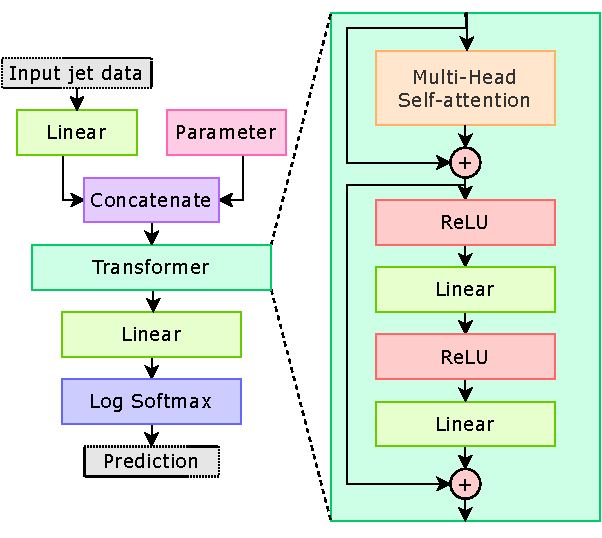
\includegraphics[trim={0cm 0cm 0cm 0cm}, width=0.45\textwidth, center]{models/constituent_net_simplified.pdf}
  \caption{Diagram with an overview of the ultra-low latency architecture.}
  \label{fig:constituent-net-simplified}
\end{figure}


\section{Accuracy-Focused Architecture}
\indo{State the goal and recap the constituent net dataset}
\indo{Talk about big value range of inputs and how we cannot preprocess unless it becomes part of the system (which it does for example to combat numerical instability)}
\indo{Mention how data could be preprocessed in general and reason most methods are too slow/not worth it}
\indo{|}
\indo{|}

\subsection{Simplification and Tuning}
\indo{List optimizations/simplifications and why they happened, back as much as possible with dataset and being hardware-aware}
\indo{stability issues solved by more normalization (coming from wide range of inputs of 30x16)}
\indo{splitting QKV into 3 separate mults}
\indo{|}
\indo{|}
\indo{|}
\indo{|}
\indo{|}

\subsection{Summary}
\indo{Short summary and pointing to diagram}
\indo{|}
\indo{|}

\begin{figure}[hpt!]
  \centering
  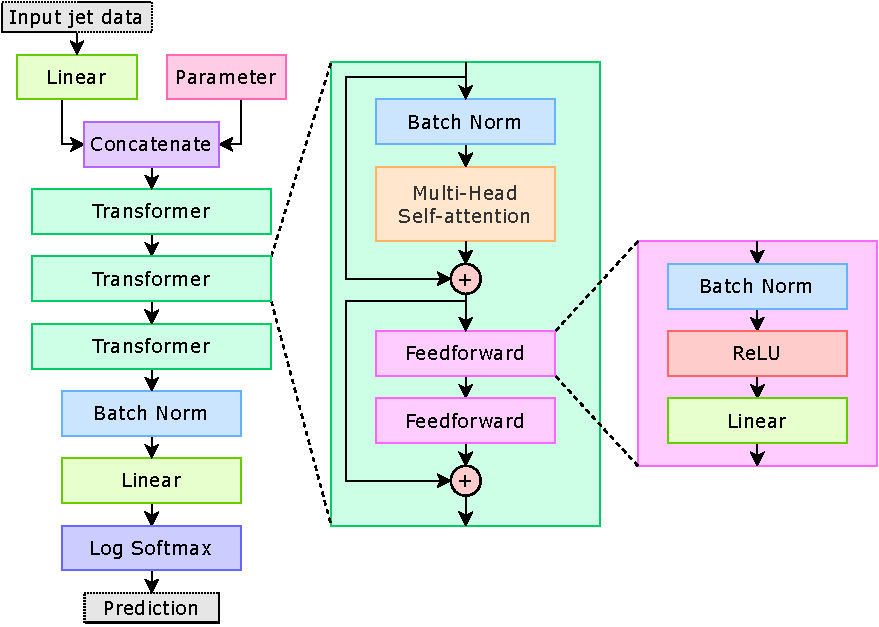
\includegraphics[trim={0cm 0cm 0cm 0cm}, width=0.6\textwidth, center]{models/constituent_net_accuracy.pdf}
  \caption{Diagram with an overview of the accuracy-focused architecture.}
  \label{fig:constituent-net-accuracy}
\end{figure}


\section{Pre-training Quantization}
\indo{Explain what it is and why we do pre-training quantization}
\indo{|}
\indo{|}
\indo{Mention PyTorch Eager Mode and PyTorch FX Graph Mode, give some explanation and show what they can and cannot, overall they are too experimental and cannot support transformer yet}
\indo{|}
\indo{|}
\indo{|}
\indo{|}
\indo{Mention Brevitas, how it compares to PyTorch}
\indo{|}
\indo{Mention QPyTorch, how it compares to PyTorch, Brevitas and why it is the best here}
\indo{|}
\indo{|}
\indo{Mention post-training quantization explained in the next chapter}

